\documentclass[border=6pt]{standalone}
\usepackage{tikz}
\usepackage[edges]{forest}
\usetikzlibrary{arrows.meta,positioning,calc,decorations.pathreplacing,shapes.geometric}
\begin{document}
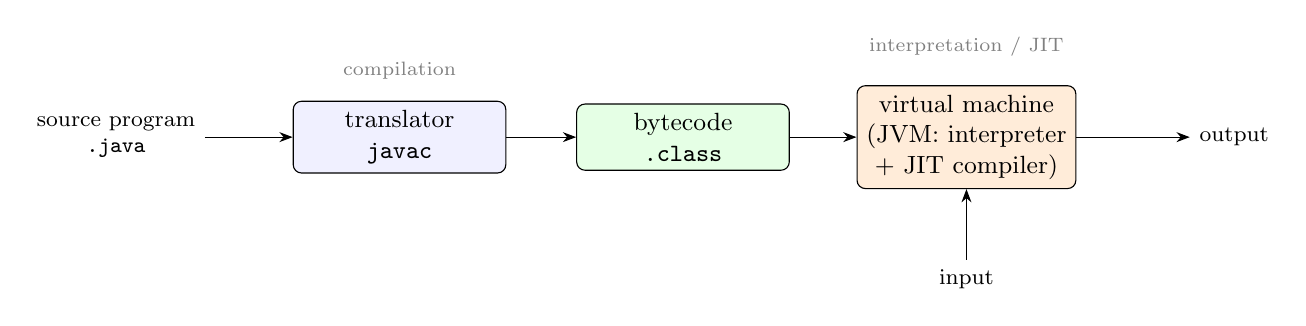
\begin{tikzpicture}[>=Stealth,font=\small,node distance=0.7cm,
 blk/.style={draw,rounded corners=3pt,minimum width=2.7cm,minimum height=0.8cm,align=center,fill=blue!6},
 io/.style={align=center,font=\footnotesize}]
\node[io] (src) at (0,0) {source program\\\texttt{.java}};
\node[blk] (jc) at (3.6,0) {translator\\\texttt{javac}};
\node[blk,fill=green!10] (bc) at (7.2,0) {bytecode\\\texttt{.class}};
\node[blk,fill=orange!15] (vm) at (10.8,0) {virtual machine\\(JVM: interpreter\\$+$ JIT compiler)};
\node[io] (out) at (14.2,0) {output};
\node[io] (inp) at (10.8,-1.8) {input};
\draw[->] (src)--(jc); \draw[->] (jc)--(bc); \draw[->] (bc)--(vm); \draw[->] (vm)--(out); \draw[->] (inp)--(vm);
\node[font=\scriptsize,gray] at (3.6,0.85) {compilation}; \node[font=\scriptsize,gray] at (10.8,1.15) {interpretation / JIT};
\end{tikzpicture}
\end{document}
